\documentclass[authoryear,preprint,review,12pt]{elsarticle}

\usepackage{amsmath}

\begin{document}

\begin{frontmatter}
\journal{Chemical Geology}
\title{Multi-sample comparison of detrital age distributions}
\author{Pieter Vermeesch}
\address{
University College London\\
Gower Street, London WC1E 6BT\\
+44 (0)20 7679 2418\\
\texttt{p.vermeesch@ucl.ac.uk}
}

\begin{abstract}
The petrography and geochronology of detrital minerals form rich
archives of information pertaining to the provenance of siliclastic
sediments. The composition and age spectra of multi-sample datasets
can be used to trace the flow of sediments through modern and ancient
sediment routing systems. Such studies often involve dozens of samples
comprising thousands of measurements. Objective interpretation of such
large datasets can be challenging and greatly benefits from
dimension-reducing exploratory data analysis tools. Principal
Components Analysis (PCA) is a proven method that has been widely used
in the context of compositional data analysis and traditional heavy
mineral studies. Unfortunately, PCA cannot be readily applied to
geochronological data, which are rapidly overtaking petrographic
techniques as the method of choice for large scale provenance
studies. This paper proposes another standard statistical technique
called Multidimensional Scaling (MDS) as an appropriate tool to fill
this void.  MDS is a robust and flexible superset of PCA which makes
fewer assumptions about the data.  Given a table of pairwise
`dissimilarities' between samples, MDS produces a `map' of points on
which `similar' samples cluster closely together, and `dissimilar'
samples plot far apart.  It is shown that the statistical effect size
of the Kolmogorov-Smirnov test is a viable dissimilarity measure. This
is not the case for the p-values of this and other tests.  To aid in
the adoption of the method by the geochronological community, this
paper includes some simple code using the statistical programming
language \texttt{R}. More extensive software tools are provided on
\verb#http://mudisc.london-geochron.com#.

\end{abstract}
\end{frontmatter}

\section{Introduction}
\label{sec:introduction}

\begin{figure}
\includegraphics[height=.9\textheight]{MuUs.pdf}
\caption{Sample locations and Kernel Density Estimates
  \citep[KDEs,][]{vermeesch2012b} of the Chinese loess study (N =
  number of concordant ages). Samples 1-5, 7 and 9-10 -- dune sand;
  samples 6 and 8 -- Cretaceous sandstone; sample L -- Quaternary
  loess; sample Y -- fluvial sand from the Yellow River; sample T --
  compilation of proposed sources in Yellow River headwaters from
  \citet{pullen2011}.}
\label{fig:mu-us}
\end{figure}

Ever since the development of single grain U-Pb dating by (ion and
laser) microprobe analysis, the method has been applied to detrital
zircon (DZ) as a means of reconstructing the provenance of
siliciclastic rocks.  Initially, DZ geochronology was primarily used
to trace the provenance of such rocks back to individual
`protosources' or source terranes \citep{gehrels1995, pell1997}. But
in recent years, the ever-increasing throughput and ever decreasing
cost of DZ geochronology has enabled a more sophisticated kind of
applications, in which the U-Pb age distributions of multiple samples
are used as a characteristic `fingerprint' to trace the flow of zircon
grains through the sediment routing system.

This paper introduces methods that make the interpretation of such
datasets more objective, using a recently published provenance study
from China as an example. \citet{stevens2012} present a dataset
comprising ten sand(stone) samples from the Mu Us desert, a Quaternary
loess sample, a modern fluvial sand sample from the Yellow River, and
a dataset of DZ ages from the Tibetan headwaters of the Yellow River
taken from \citet{pullen2011}.  The degree of similarity between these
samples can be assessed on a qualitative basis by jointly plotting
their respective age spectra (Figure \ref{fig:mu-us}). Another
commonly used visual aid is the so-called `QQ plot', in which various
quantiles of the samples are plotted against each other, the idea
being that two samples follow an identical distribution if and only if
their quantiles plot on a 1:1-line (Figure \ref{fig:QQ}).  

\begin{figure}
%\centering
\includegraphics[width=.8\textwidth]{QQplots.pdf}
\caption{Q-Q plots of the Chinese U-Pb dataset. Blue dots represent
  the 0, 5, 10, ..., 95 and 100 percentiles (or `quantiles') of the
  samples whose names are shown on the X- and Y-axis, respectively.
  Two samples follow an identical distribution if and only if their
  percentiles fall on the 1:1-line.}
\label{fig:QQ}
\end{figure}

Both the QQ plots and the age spectra can become unwieldy if they
contain more than a dozen or so samples. For example, Figure
\ref{fig:mu-us} contains n=13 Kernel Density Estimates
\citep[KDEs,][]{vermeesch2012b} showing the probability distributions
of 2,025 single grain age estimates, while the QQ-plots in Figure
\ref{fig:QQ} form an upper triangular matrix with n(n-1)/2 = 78
pairwise comparisons.  This is simply too much information for the
human eye to process. To solve this problem, we need a `filter'
removing the redundant features of the individual distributions while
preserving and amplifying the significant differences between
them. This paper makes the case that a standard statistical technique
called Multidimensional Scaling (MDS) can be used effectively for this
purpose (Sections \ref{sec:MDS} and \ref{sec:application}).  

In addition to the DZ ages, all but one (T) of the samples in the
Chinese study were subjected to heavy mineral (HM) analysis.  With the
exception of samples 1 and 8, the HM analyses were performed on
separate aliquots from the U-Pb measurements. For samples 1 and 8, the
HM mounts were prepared by mixing leftover mineral separates from the
DZ study.  Between 201 to 419 grains were counted in the 63-250$\mu$m
size fraction of each sample, resulting in an additional 2,901
datapoints.  Part of the aim of this paper is to treat these
categorical data on an equal footing with the continuous age data in a
consistent mathematical framework (Section \ref{sec:PCA}). All the
analyses presented in this paper can be reproduced using the software
discussed in Section \ref{sec:software} and made available on
\texttt{http://mudisc.london-geochron.com}.

\section{Measuring the dissimilarity between two samples}
\label{sec:dissimilarity}

Before discussing multi-sample comparisons, it is useful to review the
underlying principles for measuring the dissimilarity ($\delta_{i,j}$)
between two samples ($i$ and $j$, say).  It is desirable for any
dissimilarity measure to fulfil the following four requirements:

\begin{align}
\delta_{i,j} & \mbox{ should independent of sample size N} & \label{eq:samplesize}\\
\delta_{i,j} &= 0 \mbox{ if } i=j \mbox{ and } \delta_{i,j} > 0 \mbox{ otherwise}
& \mbox{(nonnegativity)} \label{eq:nonnegative}\\
\delta_{i,j} &= \delta_{j,i} & \mbox{(symmetry)} \label{eq:symmetric}\\
\delta_{i,k} &\leq \delta_{i,j}  + \delta_{j,k} & \mbox{(triangle inequality)} \label{eq:triangle}
\end{align}

The first requirement is important for the Chinese loess study, as it
would be impossible to compare samples 6 (N = 58) and T (N = 772)
otherwise.  If a dissimilarity measure fulfils the remaining three
conditions, then it is said to be a `metric'. One example of such a
metric is the Euclidean distance ($d_{i,j}$). Given two R-dimensional
points $x_i = (x_i^1,x_i^2,\ldots,x_i^R)$ and $x_j =
(x_j^1,x_j^2,\ldots,x_j^R)$, the Euclidean distance is given by:

\begin{equation}
d_{i,j} = \sqrt{(x_i^1-x_j^1)^2+(x_i^2-x_j^2)^2+\ldots+(x_i^R-x_j^R)^2} 
\label{eq:euclidean}
\end{equation}

Unfortunately, the space of detrital age distributions (which is a
`function space') is not a Euclidean space. And neither is the space
of HM compositions (which is a `simplex').  Therefore, the Euclidean
distance cannot be directly applied to either DZ or HM data.  However,
HM compositions can be converted to a Euclidean space by applying a
so-called logratio transformation. Further details about this are
provided in Appendix A. Unfortunately, no such transformation exist
for geochronological data, and we can therefore not use the Euclidean
distance to compare these.  Fortunately, several alternatives are
available that also fulfil conditions
\ref{eq:samplesize}-\ref{eq:triangle}. One of these is the sample
effect size of the Kolmogorov-Smirnov (KS) test:

\begin{equation}
KS = \underset{t}{max}|F_i(t)-F_j(t)|
\label{eq:ks}
\end{equation}

where $|\cdot|$ stands for the absolute value and $F(t)$ is the
empirical cumulative distribution function (CDF):

\begin{equation}
F(t) = \mbox{(number of ages less than t)/N}
\label{eq:cdf}
\end{equation}

Note that Equation \ref{eq:ks} is identical to the well known KS
\emph{statistic} \citep{feller1948}. The difference between the terms
`statistic' and `effect size' is defined in Appendix B.  The KS
statistic is most sensitive to the region near the modes of the sample
distributions, and less sensitive to their tails.  Several
alternatives are available that fix this problem, such as the
Anderson-Darling (AD) and Cram\'{e}r-von Mises (CvM) statistics, which
are based on the squared differences between two CDFs
\citep{anderson1954, anderson1962}. However, it can be shown that
these more sophisticated measures do not fulfil the triangle
inequality (Equation \ref{eq:triangle}), causing some limitations.
Therefore, the remainder of this paper will use the KS effect size as
a dissimilarity measure.

\section{Multidimensional Scaling}
\label{sec:MDS}

Let $\delta$ be a matrix of pairwise dissimilarities between n
samples:

\begin{equation}
\delta = \left(
\begin{array}{cccc}
\delta_{1,1} & \delta_{1,2} & \ldots & \delta_{1,n} \\
\delta_{2,1} & \delta_{2,2} & \ldots & \delta_{2,n} \\
\vdots & \vdots & \delta_{i,j} & \vdots \\
\delta_{n,1} & \delta_{n,2} & \ldots & \delta_{n,n} \end{array} 
\right) 
\label{eq:delta}
\end{equation}

where $\delta_{i,j}$ is the dissimilarity between samples i and j, as
before.  And let $f(\delta_{i,j})$ be a monotonically increasing
function transforming the dissimilarities into `disparities'.  Then
MDS produces an R-dimensional (where $R \leq n$) configuration of
points {\bf x} = $\{x_1,x_2,\ldots,x_i,\ldots,x_j,\ldots,x_n\}$ with
$x_i = (x_i^1,x_i^2,\ldots,x_i^R)$ and $x_j =
(x_j^1,x_j^2,\ldots,x_j^R)$ for $1 \leq i,j \leq n$. The Euclidean
distance between any two points $x_i$ and $x_j$ in this configuration
approximates the disparities between samples i and j:

\begin{equation}
d_{i,j} \approx f(\delta_{i,j}) \label{eq:d}
\end{equation}

with $d_{i,j}$ as defined by Equation \ref{eq:euclidean}.  In this
paper, we will only consider the case where R=2, so that the
configuration {\bf x} can be plotted on a sheet of paper, like a map.
Therefore, we will use the terms `configuration' and `map'
interchangeably. In fact, one of the classic applications of MDS
involves the reconstruction of a topographic map from a table of
pairwise (Euclidean) distances between cities with the minimum
possible distortion \citep[e.g., p8-9 of][]{kruskal1978}.  

If the disparity transformation is the identity matrix (i.e.,
$f(\delta_{i,j})=\delta_{i,j}$), and if $\delta_{i,j}$ is a metric,
then the configuration {\bf x} can be found analytically by relatively
straightforward linear algebra \citep[][p.23-25]{cox2000}. This is
called \emph{classical} MDS.  If the triangle inequality (Equation
\ref{eq:triangle}) is violated, then $\delta_{i,j}$ is not a metric
but a `semi-metric'. In this case, it may still be possible to perform
an MDS analysis by considering a disparity transformation such as:

\begin{equation}
f(\delta_{i,j}) = a + b \delta_{i,j}
\label{eq:f}
\end{equation}

or any other parametric equation (e.g. exponential), so long as it
monotonically increases. This superset of classical MDS is (somewhat
confusingly) called \emph{metric} MDS. It solves for the configuration
that simultaneously determines both the distances $d_{i,j}$ and the
fit to the disparity transformation $f(\delta_{i,j})$.  In the most
general case, $f$ is allowed to take any nonparametric monotonically
increasing form such as a step function. This method is called
\emph{nonmetric} MDS, and not only allows violations of the triangle
inequality but even of the condition of symmetry (Equation
\ref{eq:symmetric}). The goal of nonmetric MDS is not to approximate
the dissimilarities themselves, but rather their relative ranks.  In
the case of non-metric MDS, the solution is not found analytically but
numerically. This is done by minimizing a so-called `stress parameter'
S, the most common form (so-called `Stress-1') of which is
\citep{kruskal1964}:

\begin{equation}
\mbox{S} = \sqrt{\frac{\sum_{i=1}^{n}\sum_{j=i+1}^{n}
[f(\delta_{i,j})-d_{i,j}]^2}
{\sum_{i=1}^{n}\sum_{j=i+1}^{n}d_{i,j}^2}}\\
\label{eq:stress}
\end{equation}

The final stress value can be used to evaluate the quality of the MDS
fit (Table \ref{tab:gof}).

\begin{table}[ht]
\centering
\begin{tabular}{c|ccccc}
g.o.f & poor & fair & good & excellent & perfect\\
S & 0.2 & 0.1 & 0.05 & 0.025 & 0
\end{tabular}
\caption{Rules of thumb for interpreting the goodness of fit (g.o.f.)
  using the final value of \citet{kruskal1964}'s Stress-1 (S).}
\label{tab:gof}
\end{table}

MDS is generally insensitive to the choice of S and f. Therefore,
metric and nonmetric MDS will generally give similar-looking results,
and even the choice of $\delta_{i,j}$ will often have only a minor
effect.  This robustness is one of the major strengths of the method.

\section{Application to the Chinese dataset}
\label{sec:application}

Let us now return to the Chinese dataset to illustrate these
theoretical concepts with a practical example.  The matrix of
KS dissimilarities (multiplied with 100 for brevity) is given by:

\begin{equation}
\delta = \bordermatrix{
~ & 1 & 2 & 3 & 4 & 5 & 6 & 7 & 8 & 9 & 10 & L & T & Y\cr
1 & 0 & 14 & 33 & 27 & 18 & 14 & 15 & 22 & 48 & 32 & 42 & 37 & 40 \cr
2 & 14 & 0 & 36 & 33 & 16 & 14 & 15 & 24 & 46 & 32 & 47 & 42 & 43 \cr
3 & 33 & 36 & 0 & 19 & 24 & 44 & 47 & 55 & 17 & 10 & 13 & 12 & 8 \cr
4 & 27 & 33 & 19 & 0 & 20 & 38 & 41 & 48 & 28 & 14 & 21 & 17 & 16 \cr
5 & 18 & 16 & 24 & 20 & 0 & 22 & 24 & 33 & 31 & 20 & 33 & 28 & 30 \cr
6 & 14 & 14 & 44 & 38 & 22 & 0 & 14 & 24 & 52 & 41 & 52 & 48 & 49 \cr
7 & 15 & 15 & 47 & 41 & 24 & 14 & 0 & 16 & 51 & 43 & 54 & 49 & 52 \cr
8 & 22 & 24 & 55 & 48 & 33 & 24 & 16 & 0 & 61 & 53 & 63 & 59 & 62 \cr
9 & 48 & 46 & 17 & 28 & 31 & 52 & 51 & 61 & 0 & 20 & 22 & 18 & 16 \cr
10 & 32 & 32 & 10 & 14 & 20 & 41 & 43 & 53 & 20 & 0 & 17 & 15 & 13 \cr
L & 42 & 47 & 13 & 21 & 33 & 52 & 54 & 63 & 22 & 17 & 0 & 10 & 11 \cr
T & 37 & 42 & 12 & 17 & 28 & 48 & 49 & 59 & 18 & 15 & 10 & 0 & 7 \cr
Y & 40 & 43 & 8 & 16 & 30 & 49 & 52 & 62 & 16 & 13 & 11 & 7 & 0
}
\label{eq:deltamuus}
\end{equation}

Note that this is a symmetric matrix (due to Equation
\ref{eq:symmetric}) with zero diagonal (due to Equation
\ref{eq:nonnegative}), so that it suffices to provide the MDS
algorithm with only the upper (or lower) triangular part of it.  Using
metric MDS, the data can be completely described (i.e. S=0) by an
8-dimensional (i.e., R=8) configuration (again multiplied with 100):

\begin{equation}
{\bf x} = 
\begin{array}{c}
~ \\
1 \\
2 \\
3 \\
4 \\
5 \\
6 \\
7 \\
8 \\
9 \\
10 \\
L \\
T \\
Y 
\end{array}
\left\{
\begin{array}{cccc|cccccccc}
 && x^1 & x^2 & x^3 & x^4 & x^5 & x^6 & x^7 & x^8 & \\
1 && -17 & 10.0 & -1.9 & 2.6 & -2.2 & 1.1 & 1.2 & 0.63 & \\
2 && -19 & -2.0 & 7.4 & -2.4 & -5.2 & 0.1 & 0.8 & -0.39 \\
3 && 17 & 0.1 & 2.2 & 2.8 & -6.9 & 2.0 & -1.6 & 0.19 \\
4 && 9 & 7.0 & -4.0 & -8.4 & 3.2 & 0.1 & 0.9 & -0.93 \\
5 && -5 & -3.8 & 1.7 & -2.6 & 2.8 & -1.2 & -2.9 & 2.58 \\
6 && -25 & 2.1 & 8.2 & 2.6 & 6.4 & 1.3 & -2.6 & -0.45 \\
7 && -28 & -4.7 & -1.6 & 4.1 & 2.1 & -2.3 & 4.0 & -1.51 \\
8 && -37 & -2.7 & -10.3 & -2.2 & -3.0 & 0.9 & -1.9 & 0.13 \\
9 && 23 & -16.2 & -2.6 & 0.3 & 1.3 & 1.0 & 0.2 & -0.31 \\
10 && 14 & 0.1 & 5.9 & -3.3 & -2.0 & -4.1 & 2.0 & 1.03 \\
L && 25 & 5.1 & -4.1 & 4.0 & -0.1 & -4.6 & -3.1 & -1.44 \\
T && 21 & 3.4 & -3.3 & 3.6 & 2.6 & 2.0 & 2.6 & 2.84 \\
Y && 23 & 1.6 & 2.3 & -1.1 & 0.9 & 3.7 & 0.3 & -2.37
\end{array}
\right\}
\label{eq:xmuus}
\end{equation}

\begin{figure}
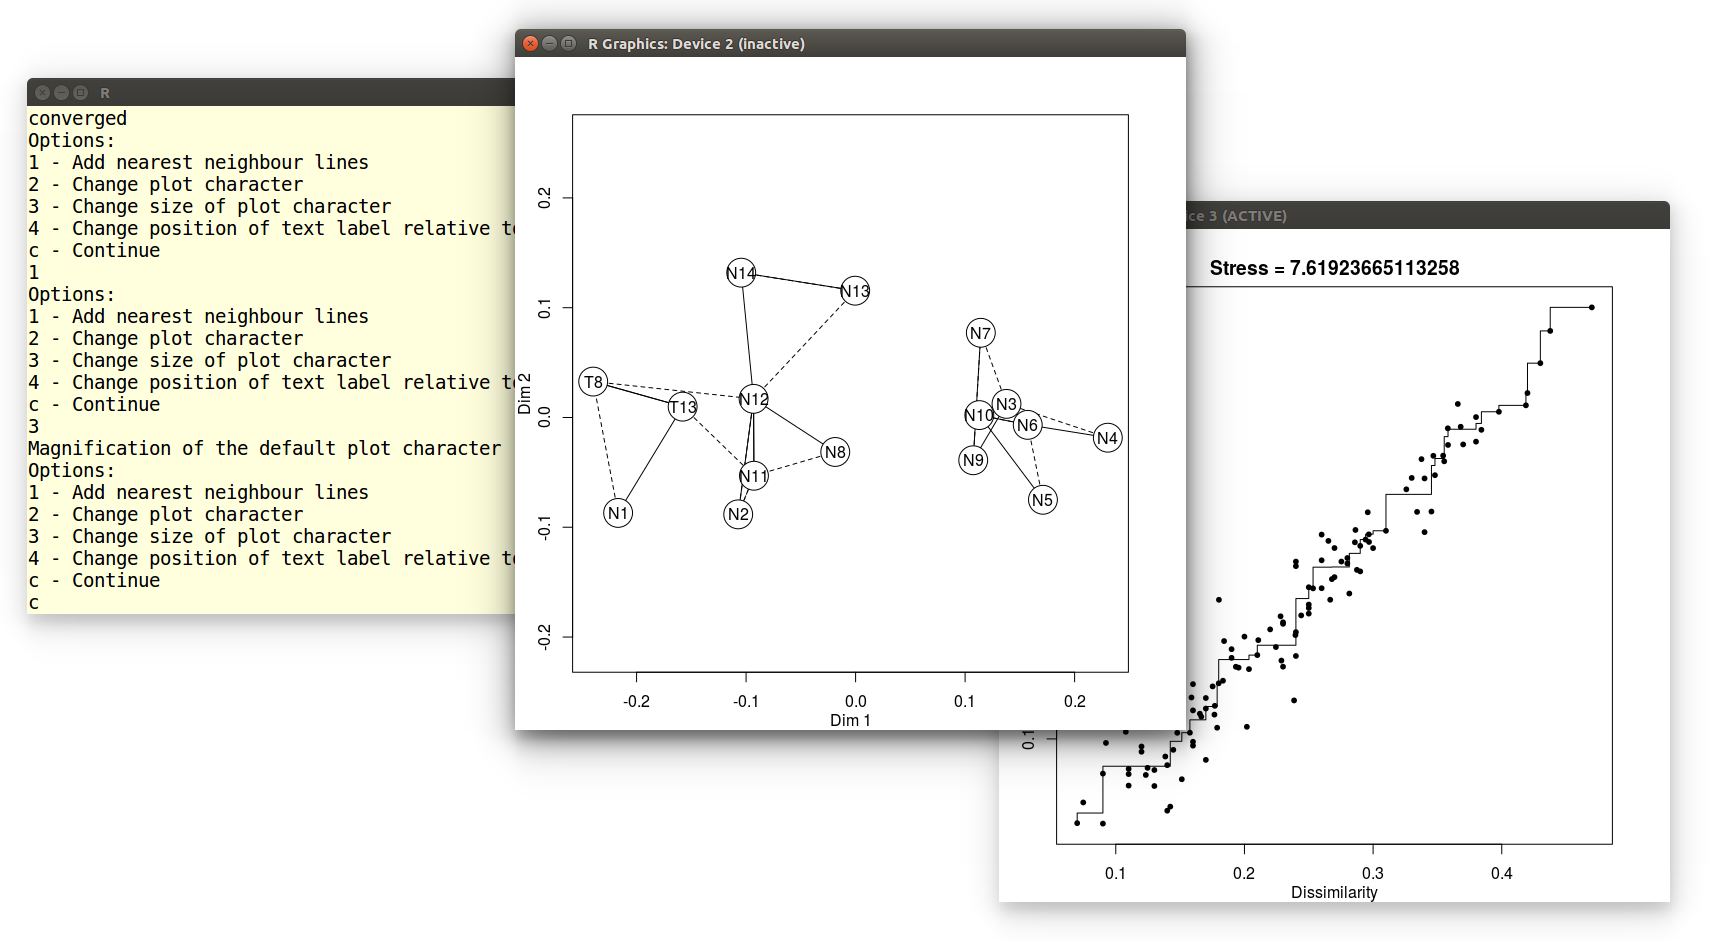
\includegraphics[width=\textwidth]{MDS.pdf}
\caption{(a) metric and (b) non-metric MDS plots of the Chinese U-Pb
  dataset using the KS effect size as a dissimilarity measure. Solid
  lines mark closest neighbours and dashed lines second closest
  neighbours.  (c) and (d) are the corresponding Shepard plots.  Both
  metric and non-metric MDS solve for the configuration that
  determines both the distances $d_{i,j}$ (blue circles) and the fit
  to the disparity transformation $f(\delta_{i,j})$ (red circles and
  lines) between all 78 possible sample pairs.  The squared and
  normalised differences between the distances and disparities
  determines the stress S (Equation \ref{eq:stress}), the final values
  of which indicate a `good' fit (S = 0.064) for the metric MDS, and
  an `excellent' fit (S = 0.025) for the nonmetric MDS (Table
  \ref{tab:gof}).}
\label{fig:MDS}
\end{figure}

The two-dimensional map coordinates are given by the first two columns
and are shown in Figure \ref{fig:MDS}a. Plugging these coordinates
into Equation \ref{eq:euclidean} and calculating the corresponding
(Euclidean) distance matrix yields:

\begin{equation}
d = \bordermatrix{
~ & 1 & 2 & 3 & 4 & 5 & 6 & 7 & 8 & 9 & 10 & L & T & Y\cr
1 & 0 & 12 & 35 & 26 & 18 & 11 & 18 & 23 & 48 & 32 & 42 & 38 & 41 \cr
2 & 12 & 0 & 36 & 30 & 14 & 7 & 9 & 18 & 44 & 33 & 45 & 40 & 43 \cr
3 & 35 & 36 & 0 & 10 & 23 & 42 & 45 & 54 & 17 & 3 & 9 & 5 & 7 \cr
4 & 26 & 30 & 10 & 0 & 18 & 35 & 39 & 47 & 27 & 8 & 16 & 12 & 15 \cr
5 & 18 & 14 & 23 & 18 & 0 & 21 & 22 & 31 & 31 & 20 & 32 & 27 & 29 \cr
6 & 11 & 7 & 42 & 35 & 21 & 0 & 7 & 13 & 51 & 39 & 50 & 46 & 48 \cr
7 & 18 & 9 & 45 & 39 & 22 & 7 & 0 & 9 & 52 & 42 & 54 & 49 & 51 \cr
8 & 23 & 18 & 54 & 47 & 31 & 13 & 9 & 0 & 61 & 50 & 62 & 58 & 60 \cr
9 & 48 & 44 & 17 & 27 & 31 & 51 & 52 & 61 & 0 & 19 & 21 & 20 & 18 \cr
10 & 32 & 33 & 3 & 8 & 20 & 39 & 42 & 50 & 19 & 0 & 12 & 8 & 10 \cr
L & 42 & 45 & 9 & 16 & 32 & 50 & 54 & 62 & 21 & 12 & 0 & 5 & 4 \cr
T & 38 & 40 & 5 & 12 & 27 & 46 & 49 & 58 & 20 & 8 & 5 & 0 & 3 \cr
Y & 41 & 43 & 7 & 15 & 29 & 48 & 51 & 60 & 18 & 10 & 4 & 3 & 0
}
\label{eq:dmuus}
\end{equation}

which is again a symmetric matrix with zero diagonal because the
Euclidean distance is a metric and therefore obeys Equations
\ref{eq:nonnegative}-\ref{eq:triangle}. Plotting the (upper- or lower
triangular parts of the) distance matrix d (Equation \ref{eq:dmuus})
against the corresponding dissimilarities $\delta$ (Equation
\ref{eq:deltamuus}) yields a so-called `Shepard plot', allowing a
graphical assessment of the quality of the model fit (Figure
\ref{fig:MDS}b).  Doing the same exercise with nonmetric MDS yields a
very similar looking map (Figure \ref{fig:MDS}c), with the fitted
distances on the Shepard plot, of course, not following a linear but a
step function (Figure \ref{fig:MDS}d).  Both Shepard plots show a
tight fit of the distances around the disparities. The relatively
minor amount of scatter is reflected in the stress values of 0.064 and
0.025. Using the rules of thumb given in Table \ref{tab:gof}, this
qualifies as a `good' fit for the metric, and an `excellent' fit for
the nonmetric MDS, respectively.\\

The MDS maps group samples with similar age spectra, and pull apart
samples with different spectra. For example, samples T (Tibet) and Y
(Yellow River) nearly overlap on the MDS maps because the KS
dissimilarity between them is only 0.07, which the smallest value in
Equation \ref{eq:deltamuus}.  On the other hand, samples L (loess) and
8 (northeastern Mu-Us) plot very far part apart on the MDS map because
the KS dissimilarity between them is 0.63, which is the largest value
in Equation \ref{eq:deltamuus}. One simple but effective way to aid in
the interpretation of MDS maps is to draw a solid line from each point
in the configuration to its `closest' neighbour in
dissimilarity-space, and a dotted line to the second closest
neighbour. For example, sample 8 is the closest (or `least
dissimilar') to sample 7 (KS=0.16), and the second closest to sample 1
(KS=0.22), while sample 7 is the closest to sample 6 (KS=0.14) and
second closest to sample 2 (KS=0.15). These connecting lines define
two distinct groups dividing the field area into a southwestern area
containing sediments of `Yellow River affinity' (samples 3, 4, 9, 10,
L, T and Y) and a northeastern area containing sediments of a
different origin (samples 1, 2, 5, 6, 7 and 8).  The MDS maps reveal a
pronounced East-West dichotomy within the Mu-Us sand desert, in which
sands from the eastern part of the desert are locally derived, whereas
the western sands are far travelled and exhibit virtually identical
age spectra to the fluvial sands of the Yellow River, which in turn
are indistinguishable from Quaternary loess of the Chinese Loess
Plateau. This leads to two new conclusions.  First, the northern parts
of the Tibet Plateau are the `ultimate source' of the Chinese
loess. Second, fluvial transport is a more significant supplier of
silt-sized particles to the Chinese loess deposits than was previously
recognised \citep{stevens2012}.

\section{Relationship with Principal Components Analysis (PCA)}
\label{sec:PCA}

Principal Components Analysis (PCA) is one of the most widely used
dimension-reducing exploratory data analysis tools for compositional
data such as HM counts.  Given a multi-dimensional dataset, PCA finds
an orthogonal tranformation (i.e., a rotation, reflection or both) to
define a lower-dimensional set of new variables explaining most of the
scatter in the input data.  PCA is closely related to MDS. In fact, it
can be shown that PCA is a special case of classical MDS in which the
dissimilarities are Euclidean distances. This means that
$\delta_{i,j}$ can be calculated in exactly the same way as $d_{i,j}$
in Equation \ref{eq:euclidean}.  The best way to measure the
dissimilarity between two HM compositions is the so-called `Aitchison
distance'. As mentioned in Section \ref{sec:dissimilarity} and
explained in Appendix A, this distance is calculated by first applying
a data transformation and then calculating the Euclidean distance on
the transformed data. Therefore, an MDS analysis of the Aitchison
distance is identical to a PCA of the transformed data (Figure
\ref{fig:PCA}).  One common way to visualise PCA results is as a
`biplot' which jointly shows the configuration and the endmember
compositions. This reveals that the most important differences between
the two groups are found in their epidote and amphibole contents.  The
MDS/PCA map of the HM counts has a striking resemblance to the MDS map
of the DZ ages (Figure \ref{fig:MDS}). Both maps are organised into
the same two groups.  Therefore, not only the zircons but also the
other heavy minerals exhibit the aforementioned East-West dichotomy,
indicating limited aeolian mixing within the Mu-Us desert.  Only
sample 1 has `switched groups', possibly due in part to the fact that
it was `reconstructed' from mineral separates.

\begin{figure}
%\centering
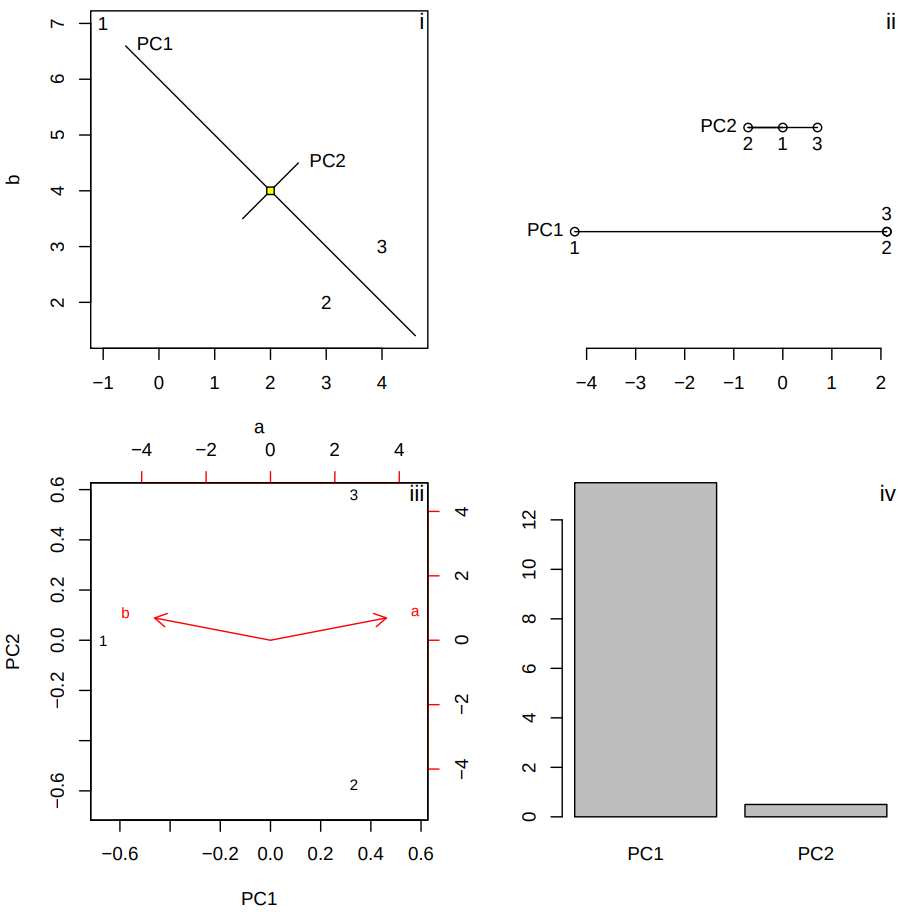
\includegraphics[width=.6\textwidth]{PCA.pdf}
\caption{Principal Components Analysis (PCA) of the
  logratio-transformed HM data from China.  This plot is identical to
  the classical MDS map of the Aitchison distances. The blue lines
  show the endmember compositions resulting from the PCA. The
  combination of the endmember compositions and the configuration is
  called a `biplot'. Asterisks mark compositions measured on mixtures
  of mineral separates rather than separate aliquots.}
\label{fig:PCA}
\end{figure}

\section{Software}
\label{sec:software}

Given that MDS is a standard statistical technique, numerous software
tools are available that can easily be adopted for detrital
geochronology, including several open source options, such as
\texttt{R} (\texttt{http://www.r-project.org}). In \texttt{R},
classical MDS is implemented by the \texttt{cmdscale} function of the
\texttt{stats} package, while nonmetric MDS is implemented by the
\texttt{isoMDS} function of the \texttt{MASS} package. Appendix C
contains a simple snippet of code using the Chinese DZ dataset as an
example.  PCA of compositional data is implemented in \texttt{R} by
the \texttt{princomp} function of the \texttt{compositions} package.
In \texttt{Matlab}, both classical, metric and non-metric MDS are
implemented by the \texttt{mdscale} function of the Statistics
Toolbox. A graphical user interface has been created that implements
this function in a user-friendly way and can be downloaded from
\texttt{http://mudisc.london-geochron.com} along with further details
about the \texttt{R} code, input files and so forth.

\section{Concluding remarks}
\label{sec:conclusions}

This paper introduced MDS as a simple yet powerful tool providing
informative, mutually consistent measures of difference for a group of
observations taken together.  It is important to note that, just like
any other dimension-reducing technique, MDS makes an abstraction of
the data and may not always represent all the details of complex
datasets. One problem with dissimilarity measures such as the KS
effect size is that they are simple scalars which cannot capture the
full richness of entire probability distributions.  For example, the
KS test cannot see the difference between a `comb-like' and a `flat'
density.  Despite these limitations, the MDS map often captures the
main features of detrital zircon datasets, as illustrated in the
Chinese case study.  

It was shown that PCA is a special case of classical MDS, using
Euclidean distance for dissimilarities and thus making restrictive
assumptions about the structure of the data, which are relaxed by
metric and non-metric MDS. Thus, MDS is a flexible technique which
makes fewer assumptions about the data than PCA. The user is not
restricted to the KS effect size used in this paper. Other
statistic-based dissimilarities such as Cram\'{e}r-von Mises and
Anderson-Darling would also work, although it is advised to use
nonmetric MDS in these cases as this is the most robust method.
Nonmetric MDS usually yields better fits than metric MDS.  In the
Chinese case study, this is reflected in the stress value of S = 0.025
for the former and S = 0.064 for the latter (Figure
\ref{fig:MDS}). The stress of the corresponding classical MDS analysis
is even higher at S = 0.78. It would therefore seem that nonmetric MDS
is the best method. However, the nonmetric MDS algorithm may fail for
small datasets. In these cases, metric and classical MDS provide a
more stable backup solution.\\

One aspect of detrital geochronology which this paper has ignored is
analytical uncertainty. An implicit assumption behind the use of the
KS effect size as a measure of dissimilarity is that all the samples
under consideration are characterised by the same analytical
precision. This is a valid assumption for the Chinese data, all of
which were measured by LA-ICP-MS (and all but one of which were
analysed in the same lab). But it is not necessarily true for datasets
combining age spectra from different laboratories using a combination
of LA-ICP-MS and SIMS, say. In such cases, it would be advised to
remove the analytical effects first.  \citet{sircombe2004a} show that
this can be achieved by adding an arbitrary variance term to all the
measurements. The resulting `Kernel Functional Estimates' (KFE) are,
essentially, over-smoothed KDEs that can be objectively compared using
the methods described in this paper.  Finally, although this paper
focused on detrital zircon U-Pb age spectra, the conclusions follow
for any other mineral (such as rutile, apatite, or monazite) or dating
technique (such as $^{40}$Ar/$^{39}$Ar, fission tracks, or
U-Th-He). In the rapidly evolving field of detrital geo- and
thermochronology, the multi-sample comparison method described here
will be able to inform more evolved efforts of the future.

\section*{Acknowledgments}

This work was funded by NERC grant \#NE/1009248/1. The author wishes
to thank Andy Carter, Matt Horstwood and Jianmei Wang for proofreading
the manuscript, and Noah McLean and an anonymous reviewer for swift
and careful reviews.

\renewcommand{\theequation}{A-\arabic{equation}}
  % redefine the command that creates the equation no.
  \setcounter{equation}{0}  % reset counter 

\section*{Appendix A: Brief summary of the Aitchison geometry applied to PCA}

Let $y = \{y_1,y_2,...,y_n\}$ be a set of k-dimensional point-counting
data $y_a=\{y_a^1,y_a^2,...,y_a^k\}$, so that $y_a^b$ represents the
integer number of grains of mineral b counted in sample a. The most
straightforward way to measure the dissimilarity between two samples
(i and j, say) would appear to be the Euclidean distance between the
corresponding proportions:

\begin{equation}
\delta_{i,j} = \sqrt{\sum_{b=1}^k
\left(\frac{y_i^b}{\sum_{c=1}^{k}y_i^c}-
\frac{y_j^b}{\sum_{c=1}^{k}y_j^c}\right)^2}
\label{eq:euclidean-proportions}
\end{equation}

Unfortunately, this approach is wrong because the proportions are
subject to a constant sum constraint (all fractions must add up to
100\%) and are therefore not mutually independent.  This restriction
produces geometric artifacts (curvature) which may negatively affect
linear procedures such as PCA.  Note that this also invalidates prior
attempts to apply PCA to detrital age histograms \citep{sircombe2000}.
To solve this problem, \citet{aitchison1982, aitchison1983,
  aitchison1986} developed a mathematical formalism in which the
compositional data are transformed to an ordinary Euclidean space
using a (centered) log-ratio transformation ($y_a^b \rightarrow
z_a^b$), by normalising the compositions to their respective geometric
means and taking logarithms:

\begin{equation}
z_a^b=ln\left(\frac{y_a^b}{\sqrt[k]{\prod_{i=1}^ky_a^i}}\right)
\label{eq:clr}
\end{equation}

with a and b referring to the sample and mineral, as before.  This
logratio transformation removes the geometric artifacts caused by the
closure operation so that the transformed data can be subjected to a
PCA. Instead of the centered logratio transformation, other options
are available such as the isometric logratio transformation (ilr),
which may actually be even better suited for PCA/MDS
\citep{egozcue2003, filzmoser2009}.

\section*{Appendix B: Why p-values are unsuitable as a measure of dissimilarity}

Some workers have used statistical tests such as Kolmogorov-Smirnov to
make the comparison of detrital age distibutions more `objective' than
mere visual inspection of age spectra or QQ-plots.  Such statistical
tests require the formulation of a so-called `null hypothesis' (e.g.,
``two detrital age distributions were drawn from the same
population''), and the selection of a `test statistic' (e.g., Equation
\ref{eq:ks}).  If the observed value of the test statistic is
`unlikely' to occur under the null hypothesis, then the latter is
rejected in favour of the alternative hypothesis (``two detrital age
distributions were drawn from different populations'').  The
probability of observing a value at least as extreme as the observed
statistic under the null hypothesis is called the `p-value'.  An
arbitrary cut-off value $\alpha$ may be used to make a decision on a
`100(1-$\alpha$)\% confidence level'. For example, if $\alpha$=0.05
and $p<\alpha$, then $H_0$ is rejected in favour of $H_a$ `with 95\%
confidence'.  The probability of erroneously rejecting a true null
hypothesis, which is given by $\alpha$, is also called a `Type-I
error'. In other words, the $\alpha$-value expresses the risk we are
willing to take of committing a Type-I error.  The p-value is a poor
measure of dissimilarity between samples, because it lumps together
two factors: the `effect size' and the `sample size'.  The sample size
is simply the total number of grains analysed (N).  The effect size
expresses {\it``the degree to which the null hypothesis is false''}
\citep{cohen1977}. To illustrate this concept, consider the case of
two Normally distributed detrital age populations with means $\mu_1$
and $\mu_2$, variances $\sigma_1^2$ and $\sigma_2^2$, and sample sizes
$N_1$ and $N_2$, respectively.  Assume that $N_1 = N_2 = N$ and
$\sigma_1 = \sigma_2 = \sigma$.  Let $\bar{X_1}$ and $\bar{X_2}$ be
the sample means and $S_1^2$ and $S_2^2$ the sample variances. We can
test the null hypothesis ``$H_o: \mu_1 = \mu_2$'' with the t-test,
using the t-statistic:

\begin{equation}
t = \frac{\bar{X_1}-\bar{X_2}}{\sqrt{(S_1^2+S_2^2)/N}}
\label{eq:t-stat1}
\end{equation}

where the denominator is the standard error of the difference between
the two means. The sample effect size of the t-test is given by:

\begin{equation}
d = \frac{\bar{X_1}-\bar{X_2}}{\sqrt{(S_1^2+S_2^2)/2}}
\label{eq:t-stat2}
\end{equation}

where the denominator is the `pooled standard deviation' of the two
samples. By definition, $d = 0$ under the null hypothesis. Let us now
consider the situation where $d \neq 0$. Suppose that $\mu_1$ = 100.1
Ma, $\mu_2$ = 100.1 Ma, and $\sigma$ = 1 Ma so that the population
effect size is 0.1. Suppose for the sake of simplicity that these
population characteristics are reflected in the sample so that $d =
0.1$. Table \ref{tab:tstat} shows some key values of the t-statistic
and corresponding p-values for different sample sizes.  Not
surprisingly, a sample size of N = 10 is insufficient to resolve the
0.1 Ma `offset' between the two peaks. In this case, the p-value is
0.41, which is greater than the cutoff value of $\alpha = 0.05$,
leading us to erroneously accept the false null hypothesis. This means
that we have committed a `Type-II error'. It is only when sample size
increases to N = 1,000 that the t-test has sufficient `power' to
reject the null hypothesis ($0.013 < \alpha$).  In conclusion, both
the statistic and the p-value of the t-test are sensitive functions of
sample size. Both are therefore unsuitable as measures of
dissimilarity in an MDS analysis.

\begin{table}[here]
\centering
\begin{tabular}{c|cccc}
N & 10 & 100 & 1,000 & 10,000\\
t & $1/\sqrt{10}$ & 1 & $\sqrt{10}$ & 100\\
p & 0.41 & 0.24 & 0.013 & $8\times10^{-13}$
\end{tabular}
\label{tab:tstat}
\caption{Statistic (t) and p-value (p) of a t-test with sample effect
  size d=0.1 as a function of sample size (N).  The strong dependence
  of t and p on N indicates that both parameters are unsuitable as
  dissimilarity measures.}
\end{table}

These same arguments are valid for other statistical tests such as
Chi-square and Kolmogorov-Smirnov, with the caveat that the effect
size of the KS-test is given by the KS-statistic itself (Equation
\ref{eq:ks}).  Nevertheless, the p-value of the KS-test is still a
function of sample size and is therefore still useless as a
dissimilarity measure.

\section*{Appendix C: Multidimensional scaling with \texttt{R}}

This section presents a simple example of computer code for MDS
analysis with the open source statistical programming language
\texttt{R}. The example input file \texttt{DZages.Rdata} containing
the data shown in Figure \ref{fig:mu-us} can be downloaded from
\texttt{http://mudisc.london-geochron.com}.

\begin{verbatim}
library(MASS)          # load the `Modern Applied Statistics with S' package
load("DZages.Rdata")   # load the dataset of U-Pb ages
n = length(DZages)     # n = the number of samples
diss = mat.or.vec(n,n) # initialize the dissimilarity matrix
for (i in 1:n){        # loop through all possible pairs of samples
 for (j in 1:n){       # calculate the kolmogorov-smirnov statistic
  diss[i,j] = ks.test(DZages[[i]],DZages[[j]])$statistic } }
cmds = cmdscale(diss)                  # classical multidimensional scaling
plot(cmds[,1],cmds[,2], type="n")      # set up the plot
text(cmds[,1],cmds[,2], names(DZages)) # label the samples by their name
dev.new()                              # open a new plot window
nmds = isoMDS(diss)                    # non-metric multidimensional scaling
plot(nmds$points[,1],nmds$points[,2], type="n")      # set up the plot
text(nmds$points[,1],nmds$points[,2], names(DZages)) # add labels
\end{verbatim}

\section*{References}
%\bibliography{../biblio} 
%\bibliographystyle{elsarticle-harv}

\begin{thebibliography}{19}
\expandafter\ifx\csname natexlab\endcsname\relax\def\natexlab#1{#1}\fi
\expandafter\ifx\csname url\endcsname\relax
  \def\url#1{\texttt{#1}}\fi
\expandafter\ifx\csname urlprefix\endcsname\relax\def\urlprefix{URL }\fi

\bibitem[{Aitchison(1982)}]{aitchison1982}
Aitchison, J., 1982. The statistical analysis of compositional data. Journal of
  the Royal Statistical Society 44, 139--177.

\bibitem[{Aitchison(1983)}]{aitchison1983}
Aitchison, J., 1983. Principal component analysis of compositional data.
  Biometrika 70~(1), 57--65.

\bibitem[{Aitchison(1986)}]{aitchison1986}
Aitchison, J., 1986. The statistical analysis of compositional data. London,
  Chapman and Hall.

\bibitem[{Anderson(1962)}]{anderson1962}
Anderson, T.~W., 1962. {On the distribution of the two sample Cr\'{a}mer - Von
  Mises criterion}. Annals Mathematical Statistics 33.

\bibitem[{Anderson and Darling(1954)}]{anderson1954}
Anderson, T.~W., Darling, D.~A., 1954. A test of goodness of fit. Journal of
  the American Statistical Association 49~(268), pp. 765--769.

\bibitem[{Cohen(1977)}]{cohen1977}
Cohen, J., 1977. {Statistical power analysis for the behavioral sciences}.
  Academic Press New York.

\bibitem[{Cox and Cox(2000)}]{cox2000}
Cox, T.~F., Cox, M. A.~A., 2000. {Multidimensional Scaling, Second Edition}.
  {Chapman \& Hall/CRC}.

\bibitem[{Egozcue et~al.(2003)Egozcue, Pawlowsky-Glahn, Mateu-Figueras, and
  Barcelo-Vidal}]{egozcue2003}
Egozcue, J., Pawlowsky-Glahn, V., Mateu-Figueras, G., Barcelo-Vidal, C., 2003.
  Isometric logratio transformations for compositional data analysis.
  Mathematical Geology 35~(3), 279--300.

\bibitem[{Feller(1948)}]{feller1948}
Feller, W., 1948. On the {K}olmogorov-{S}mirnov limit theorems for empirical
  distributions. The Annals of Mathematical Statistics 19, 177--189.

\bibitem[{Filzmoser et~al.(2009)Filzmoser, Hron, and Reimann}]{filzmoser2009}
Filzmoser, P., Hron, K., Reimann, C., 2009. Principal component analysis for
  compositional data with outliers. Environmetrics 20~(6), 621--632.

\bibitem[{{Gehrels} et~al.(1995){Gehrels}, {Dickinson}, {Ross}, {Stewart}, and
  {Howell}}]{gehrels1995}
{Gehrels}, G.~E., {Dickinson}, W.~R., {Ross}, G.~M., {Stewart}, J.~H.,
  {Howell}, D.~G., 1995. {Detrital zircon reference for Cambrian to Triassic
  miogeoclinal strata of western North America}. Geology 23, 831.

\bibitem[{Kruskal(1964)}]{kruskal1964}
Kruskal, J., 1964. Multidimensional scaling by optimizing goodness of fit to a
  nonmetric hypothesis. Psychometrika 29~(1), 1--27.

\bibitem[{Kruskal and Wish(1978)}]{kruskal1978}
Kruskal, J.~B., Wish, M., 1978. Multidimensional scaling. Vol. 07-011 of Sage
  University Paper series on Quantitative Application in the Social Sciences.
  Sage Publications, Beverly Hills and London.

\bibitem[{Pell et~al.(1997)Pell, Williams, and Chivas}]{pell1997}
Pell, S.~D., Williams, I.~S., Chivas, A.~R., 1997. The use of protolith
  zircon-age fingerprints in determining the protosource areas for some
  {A}ustralian dune sands. Sedimentary Geology 109, 233--260.

\bibitem[{Pullen et~al.(2011)Pullen, Kapp, McCallister, Chang, Gehrels,
  Garzione, Heermance, and Ding}]{pullen2011}
Pullen, A., Kapp, P., McCallister, A., Chang, H., Gehrels, G., Garzione, C.,
  Heermance, R., Ding, L., 2011. Qaidam basin and northern Tibetan plateau as
  dust sources for the Chinese loess plateau and paleoclimatic implications.
  Geology 39, 1031--1034.

\bibitem[{Sircombe(2000)}]{sircombe2000}
Sircombe, K.~N., 2000. Quantitative comparison of large sets of
  geochronological data using multivariate analysis: A provenance study example
  from {A}ustralia. Geochimica et Cosmochimica Acta 64, 1593--1616.

\bibitem[{{Sircombe} and {Hazelton}(2004)}]{sircombe2004a}
{Sircombe}, K.~N., {Hazelton}, M.~L., 2004. {Comparison of detrital zircon age
  distributions by kernel functional estimation}. Sedimentary Geology 171,
  91--111.

\bibitem[{Stevens et~al.(2012)Stevens, Carter, Watson, Lu, Vermeesch, And\'{o},
  Garzanti, Bird, and Sevastjanova}]{stevens2012}
Stevens, T., Carter, A., Watson, T., Lu, H., Vermeesch, P., And\'{o}, S.,
  Garzanti, E., Bird, A., Sevastjanova, I., 2012. {Role of the Yellow River in
  the origin of Chinese Loess Plateau dust and Mu Us desert sands}. Quaternary
  Science Reviews, (in review).

\bibitem[{Vermeesch(2012)}]{vermeesch2012b}
Vermeesch, P., 2012. On the visualisation of detrital age distributions.
  Chemical Geology 312-313, 190--194.

\end{thebibliography}

\end{document}
